Before building the robotic workcell in the real world, the kassow robot is simulated in the ROS and gazebo software environment.

\subsubsection{ROS}
\label{subsubsec:ROS}
For more information on ROS, see section \ref{subsec:ROS}. A URDF model of the KR1410 with gripper attached is created
complete with all positions of links, joints, sensors, models etc. This URDF description of robot is then ready to be tested
in the workcell. Few open-source additional packages were also used for building this simulation. For example, for attaching an
object to the finger joint which simulates a grasping action in gazebo simulator. \cite{gazebo-pkgs}

The robotic motion of unloading station gripper and the manipulation of KR1410 using the robotic gripper is simulated using ROS. (See Figure \ref{fig:gazebo-rviz})

\begin{figure}[h]
    \centering
    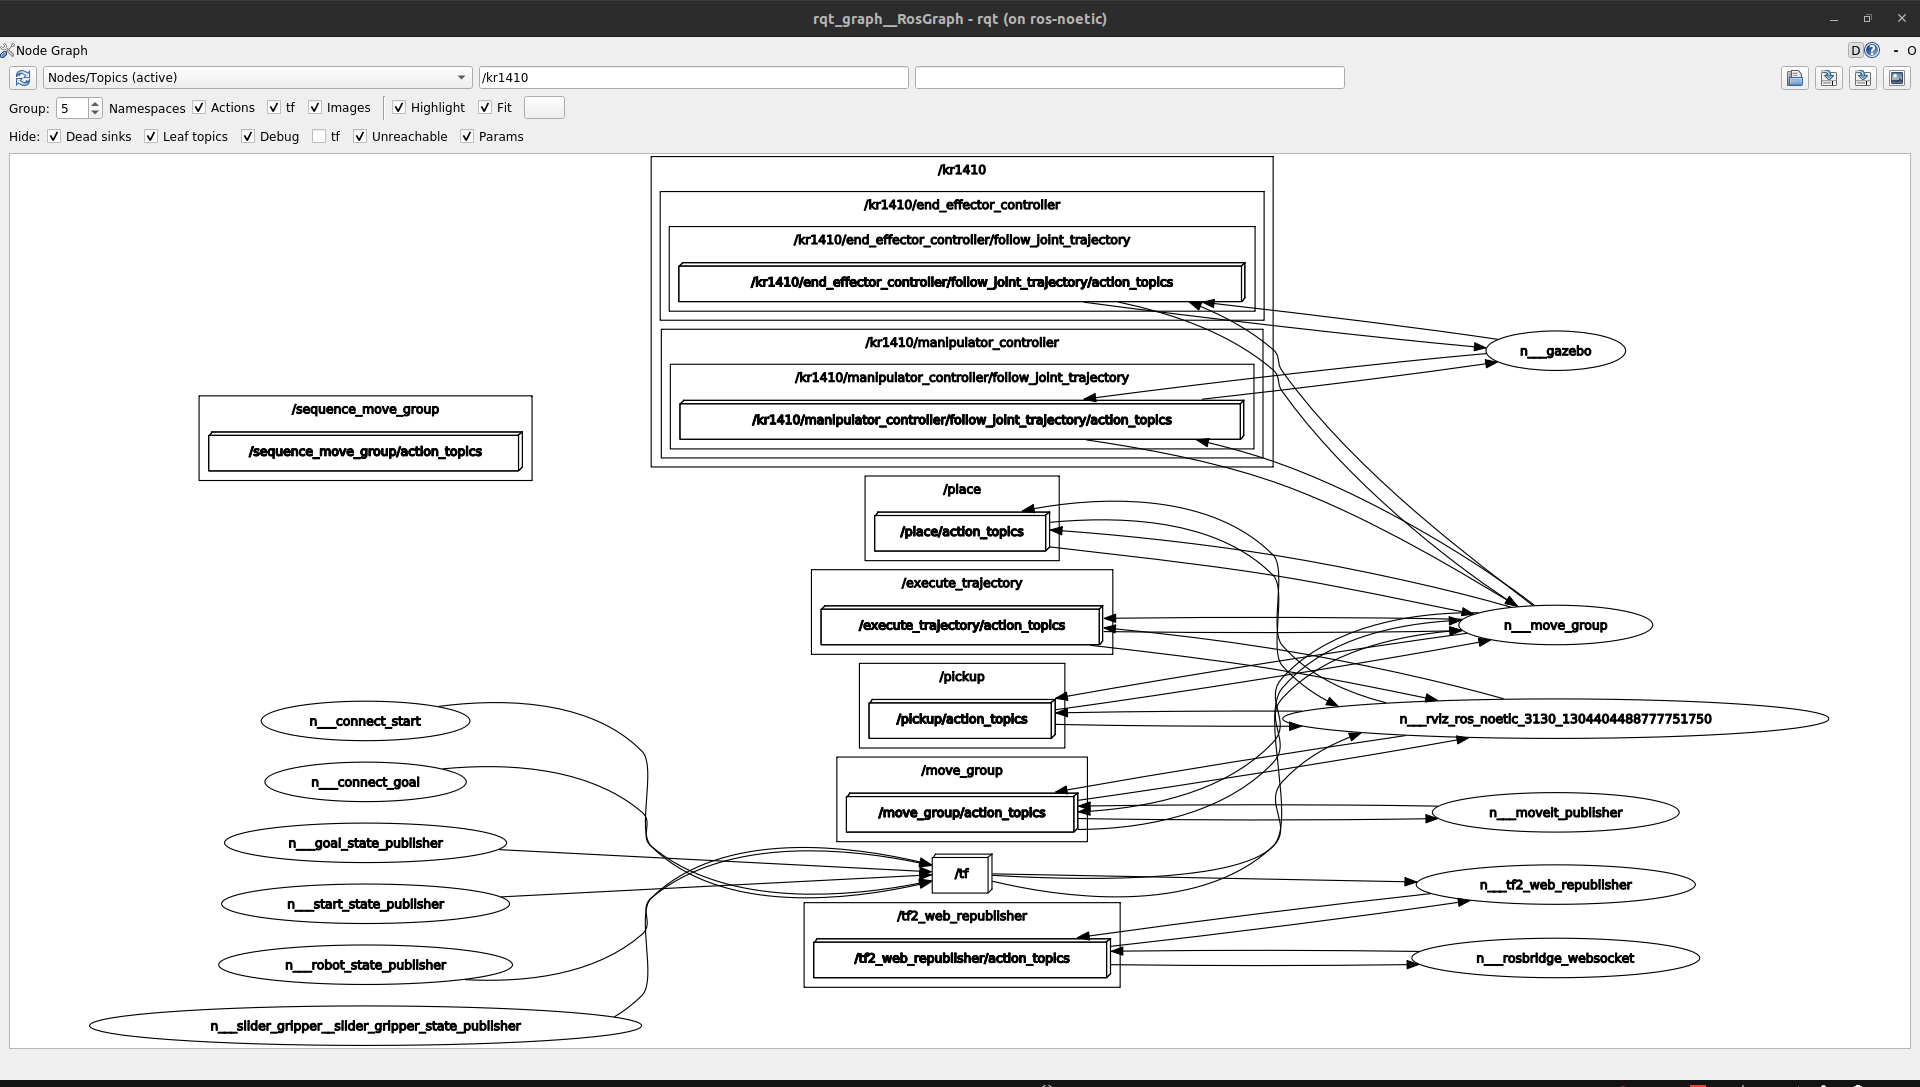
\includegraphics[width=\textwidth]{figures/rosgraph.png}
    \caption{ROSGraph}
    \label{fig:rosgraph}
\end{figure}

Many custom ROS packages \cite{rospackage} are created to simulate the workcell. A single ROS launch \cite{roslaunch} file is launched to run every node \cite{rosnode}, service \cite{rosservice} and parameter \cite{parameterserver} or action servers \cite{actionserver}
Figure \ref{fig:rosgraph} visualizes the computation graph of the simulation. It shows the currently active ROS nodes \cite{rosnode}
and topics \cite{rostopic} in the simulation of robotic workcell.


\subsubsection{Gazebo Simulator}
\label{subsubsec:gazebo}
Gazebo is a 3D dynamic simulator with the ability to accurately and efficiently simulate populations
of robots in complex indoor and outdoor environments. While similar to game engines, Gazebo
offers physics simulation at a much higher degree of fidelity, a suite of sensors, and interfaces for
both users and programs. \cite{gazebo-classic}

A model of the entire workcell is created for the gazebo simulator. The assets are converted from CAD designs
to .dae and .stl file format using blender software. These meshes are then included in the SDF model object.
The workcell is then ready to be simulated in the gazebo simulator.

\begin{figure}[h]
    \centering
    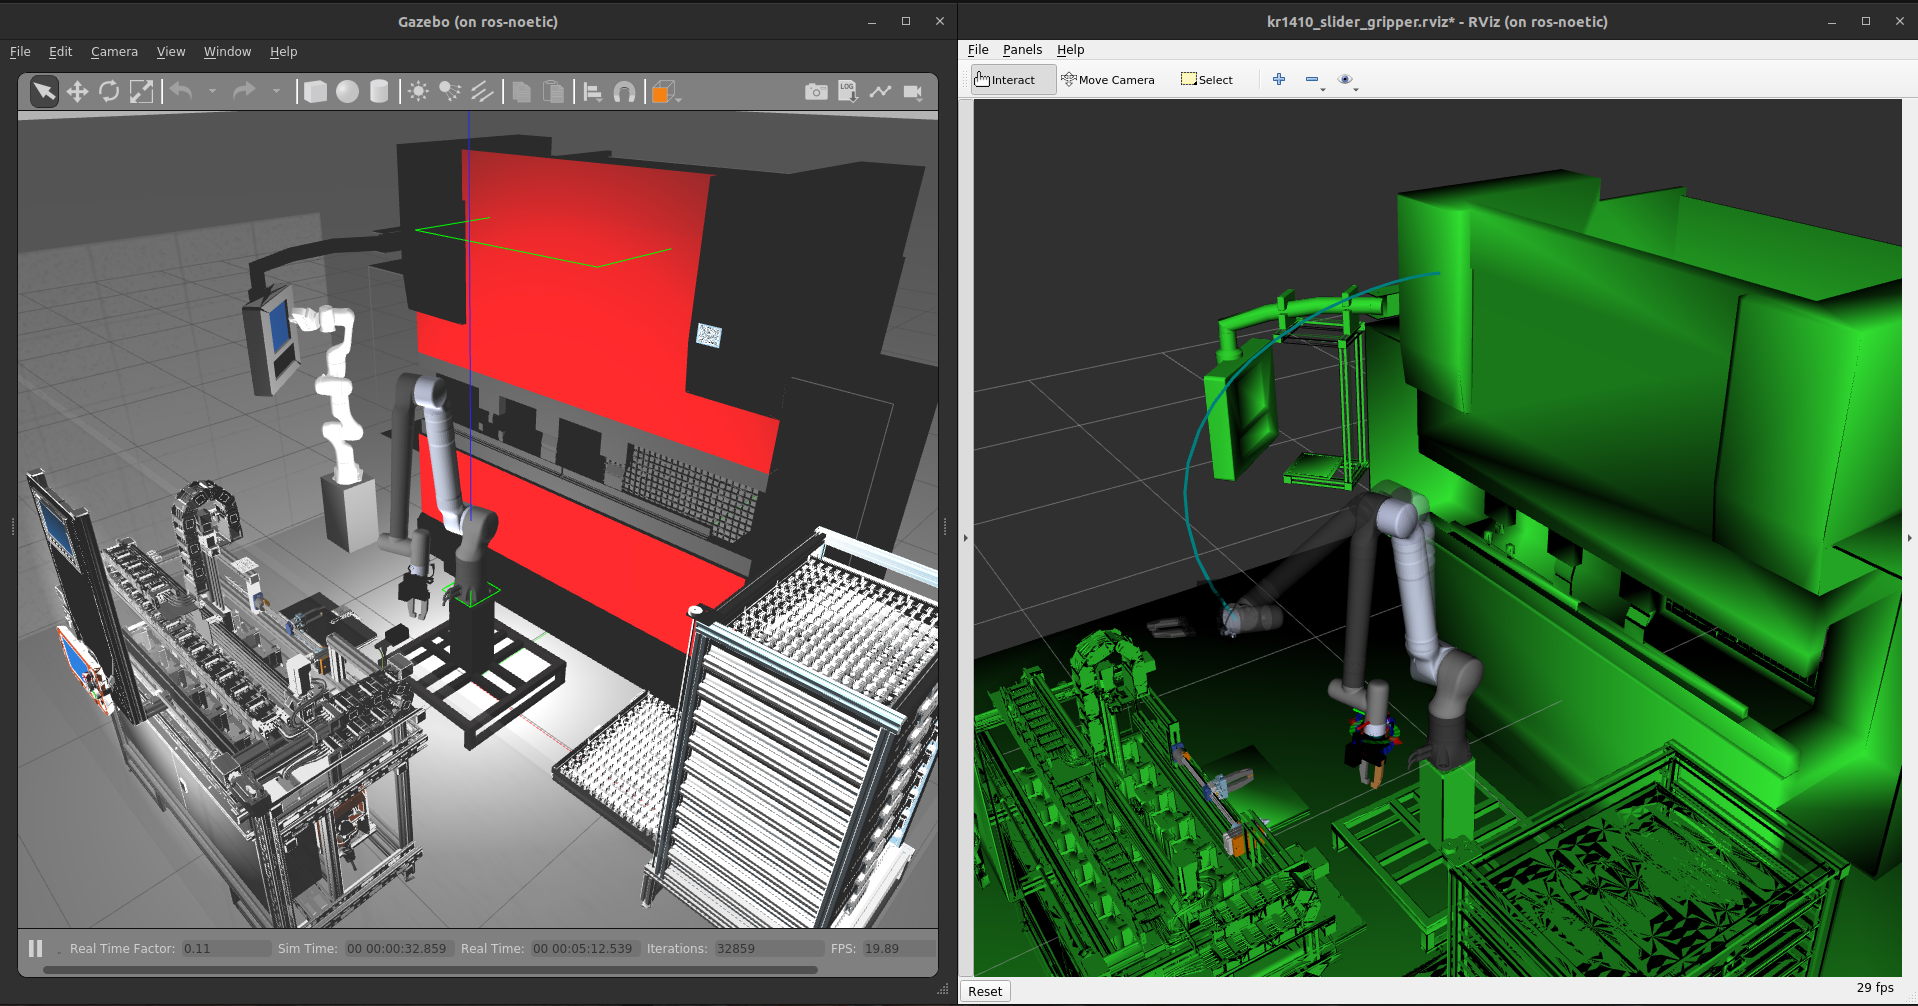
\includegraphics[width=\textwidth]{figures/gazebo-rviz.png}
    \caption{Robotic workcell in Gazebo simulator (left) and RViz (right)}
    \label{fig:gazebo-rviz}
\end{figure}

\subsubsection{RViz}
\label{subsubsec:RViz}
RViz is short for ROS Visualization. It is a 3D visualization software tool for robots, sensors, and algorithms.
It allows seeing the robot's perception of its world (real or simulated).
The purpose of RViz is to visualize the state of a robot. It uses sensor data to try
to create an accurate depiction of what is going on in the robot's environment. \cite{rviz}

\subsubsection{MoveIt}
\label{subsubsec:moveit}
MoveIt is a software for ROS used for manipulation, motion planning, 3D perception, kinematics, control and navigation. \cite{moveit}
MoveIt is used to get the solve the kinematics of the 7-axis kassow robot and do robotic manipulation and perception.
A collision mesh of the workcell is published in the planning scene as can be seen in RViz in Figure \ref{fig:gazebo-rviz}.
This makes the KR1410 to plan trajectories without any collision in the workcell. The robotic gripper is also controlled using MoveIt package.
